%%%%%%%%%%%%%%%%%%%%%%%%%%%%%%%%%%%%%%%%%%%%%%%%%%%%%%%%%%%%%%%
%                                                             %
% MIEX                                                        %
% Extracci�n de informaci�n de documentos XML mediante SP     %
%                                                             %
% Proyecto Fin de Carrera (EUITITG)                           %
% nn de Septiembre de 2007 - Gij�n                            %
%                                                             %
% Licencia GNU GPL2                                           %
%                                                             %
% Ignacio Barrientos <nacho@criptonita.com>                   %
%                                                             %
%%%%%%%%%%%%%%%%%%%%%%%%%%%%%%%%%%%%%%%%%%%%%%%%%%%%%%%%%%%%%%%

%%%%%%%%%%%%%%%%%%%%%%%%%%%%%%%%%%%%%%%%%%%%%%%%%%%%%%%%%%%%%%%%
%%%%%%%%%%%%%%%%%% Configuraci�n del entorno %%%%%%%%%%%%%%%%%%%
%%%%%%%%%%%%%%%%%%%%%%%%%%%%%%%%%%%%%%%%%%%%%%%%%%%%%%%%%%%%%%%%

% Tipo de documento LaTeX-beamer
\documentclass[14pt]{beamer}

% Acentos pasivos
\usepackage[latin1]{inputenc}
\usepackage[T1]{fontenc}
\usepackage{ulem}
\usepackage{qtree}

% Look and feel
\usetheme{Copenhagen}
\usecolortheme{rose}
%\usefonttheme{structurebold}

% Eliminar la botonera de navegaci�n
\setbeamertemplate{navigation symbols}{}

% Informaci�n de autor�a
\title{MIEX} 
\subtitle{Extracci�n de informaci�n de documentos XML mediante Stanford Parser}
\date{nn de Septiembre de 2007}
\institute
{
  \bf
  {
    Proyecto Fin de Carrera\\
    E.U.I.T. Inform�tica y Telem�tica de Gij�n
  }
}
\author{Ignacio Barrientos <nacho@debian.org>}


%%%%%%%%%%%%%%%%%%%%%%%%%%%%%%%%%%%%%%%%%%%%%%%%%%%%%%%%%%%%%%%%
%%%%%%%%%%%%%%%%%% Inicio de la presentaci�n %%%%%%%%%%%%%%%%%%%
%%%%%%%%%%%%%%%%%%%%%%%%%%%%%%%%%%%%%%%%%%%%%%%%%%%%%%%%%%%%%%%%
\begin{document}

%-------------------------- SLIDE ---------------------------%

\frame
{
  % Portada
  \titlepage
}

%-------------------------- SLIDE ---------------------------%

\frame
{
  % Solo interesan las secciones para el �ndice
  \setcounter{tocdepth}{1}
  % Creamos tabla de contenidos
  \tableofcontents
}

%%%%%%%%%%%%%%%%%%%%%%%%%%%%%%%%%%%%%%%%%%%%%%%%%%%%%%%%%%%%%%%%%%%%%%%%%
% Introducci�n                                                          %
%%%%%%%%%%%%%%%%%%%%%%%%%%%%%%%%%%%%%%%%%%%%%%%%%%%%%%%%%%%%%%%%%%%%%%%%%

\section{Introducci�n}

\frame
{
  \setcounter{tocdepth}{1}
  \tableofcontents[currentsection]
}

%-------------------------- SLIDE ---------------------------%

\frame
{

  \frametitle{El Stanford Parser}

  \begin{itemize}
  \item Stanford Natural Language Processing Group\footnote{http://nlp.stanford.edu/}
  \item Analizador de lenguaje natural
  \item Sint�ctico + Sem�ntico
  \item Java (J2SE)
  \end{itemize}

  \begin{center}
  \begin{block}{Objetivo principal}<2->
    \begin{large}
      \begin{center}
      Cubrir las carencias de usabilidad del programa para un problema
      en concreto.
      \end{center}
    \end{large}
  \end{block}
  \end{center}
}

%-------------------------- SLIDE ---------------------------%

\frame
{
  \frametitle{Ejemplo de metadatos generados}

  \begin{itemize}
    \item Parse tree
    \item Dependencias entre palabras
  \end{itemize}

  \begin{block}{Oraci�n objetivo}
    \begin{center}
      The Debian Project is an association of individuals
    \end{center}
  \end{block}
}


%-------------------------- SLIDE ---------------------------%

\frame
{
  \frametitle{Parse tree}

  \begin{center}
  \begin{scriptsize}
  \Tree[.ROOT [.S [.NP [.DT The ] [.NNP Debian ] [.NNP Project ] ] [.VP
  [.VBZ is ] [.NP [.NP [.DT an ] [.NN association ] ] [.PP [.IN of ] [.NP [.NNS individuals ] ] ] ] ] ] ]
  \end{scriptsize}
  \end{center}
}


%-------------------------- SLIDE ---------------------------%

\frame
{
  \frametitle{Dependencias\footnote{http://nlp.stanford.edu/pubs/LREC06\_dependencies.pdf} entre palabras}

  \begin{enumerate}
    \item det(Project-3, The-1)
    \item nn(Project-3, Debian-2)
    \item nsubj(association-6, Project-3)
    \item cop(association-6, is-4)
    \item det(association-6, an-5)
    \item prep\_of(association-6, individuals-8)
  \end{enumerate}
}

%-------------------------- SLIDE ---------------------------%

\frame
{
  \frametitle{La cara amigable del Stanford Parser...}

  \begin{figure}[h]
    \begin{center}
      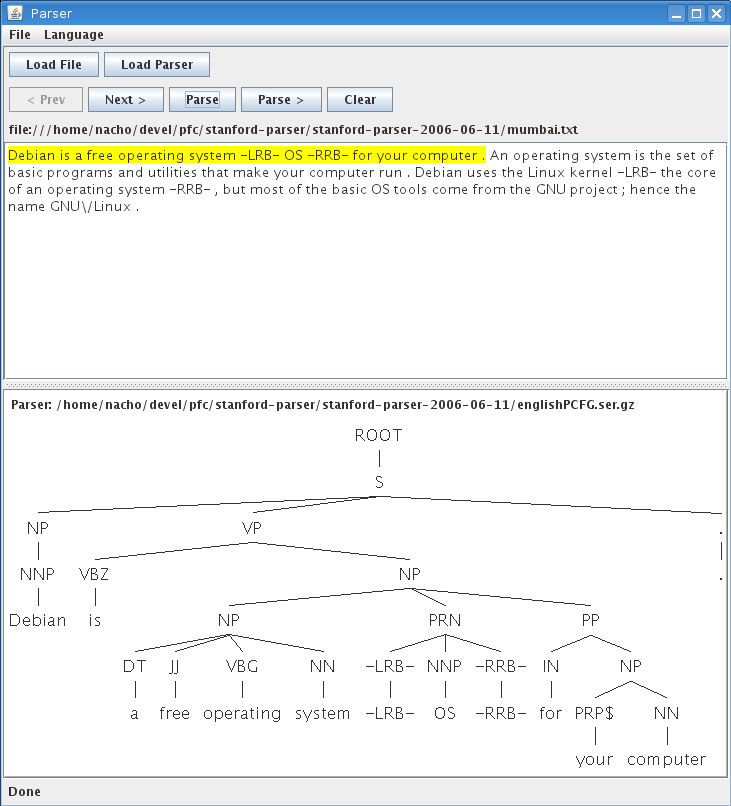
\includegraphics[scale=0.3]{images/spui.png}
    \end{center}
  \end{figure}
}

%-------------------------- SLIDE ---------------------------%

\frame
{
  \frametitle{... y la cara m�s usual}

  \begin{figure}[h]
    \begin{center}
      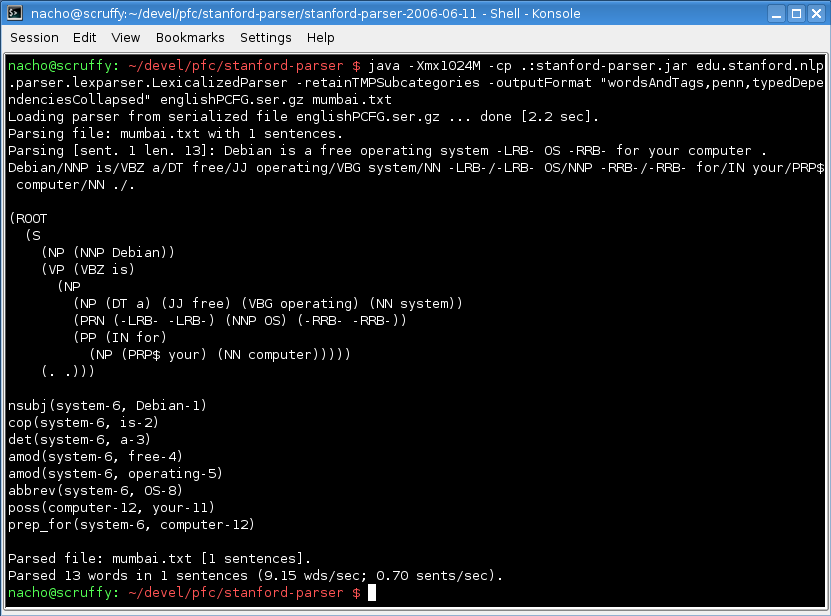
\includegraphics[scale=0.4]{images/spconsole.png}
    \end{center}
  \end{figure}
}

%-------------------------- SLIDE ---------------------------%

\frame
{
  \frametitle{Carencias del analizador}

    \begin{itemize}
      \item<1-> Pobre tratamiento de ficheros XML
      \item<2-> Manejo tedioso y \textit{poco amigable}
      \item<3-> El almacenamiento no es \textbf{flexible}
    \end{itemize}
}

%-------------------------- SLIDE ---------------------------%

\frame
{
  \frametitle{L�neas de trabajo}
  
  \begin{block}{Entrada}<1->
    \begin{itemize}
      \item<1-> Enriquecer el tratamiento de XML + validaci�n 
      \item<1-> Configurable f�cilmente
      \item<2- | alert@2-> .conf + l�nea de comandos simple + schema
    \end{itemize}
  \end{block}

  \begin{block}{Salida}<3->
    \begin{itemize}
      \item<3-> No \textit{final}
      \item<3-> Flexible
      \item<4- | alert@3-> Base de datos
    \end{itemize}
  \end{block}
}

%%%%%%%%%%%%%%%%%%%%%%%%%%%%%%%%%%%%%%%%%%%%%%%%%%%%%%%%%%%%%%%%%%%%%%%%%
% Funcionamiento                                                        %
%%%%%%%%%%%%%%%%%%%%%%%%%%%%%%%%%%%%%%%%%%%%%%%%%%%%%%%%%%%%%%%%%%%%%%%%%

\section{Funcionamiento}

\frame
{
  \setcounter{tocdepth}{1}
  \tableofcontents[currentsection]
}

%-------------------------- SLIDE ---------------------------%

\frame
{
  \frametitle{�C�mo funciona?}

  \begin{figure}[h]
    \begin{center}
      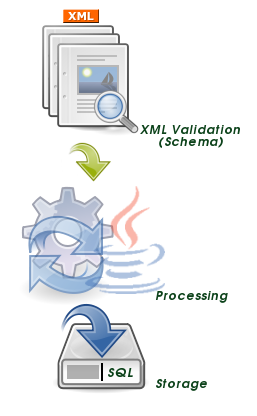
\includegraphics[scale=0.8]{images/miex.png}
    \end{center}
  \end{figure}
}

%-------------------------- SLIDE ---------------------------%

\frame
{
  \frametitle{�M�s detalle, por favor!}

  \begin{figure}[h]
    \begin{center}
      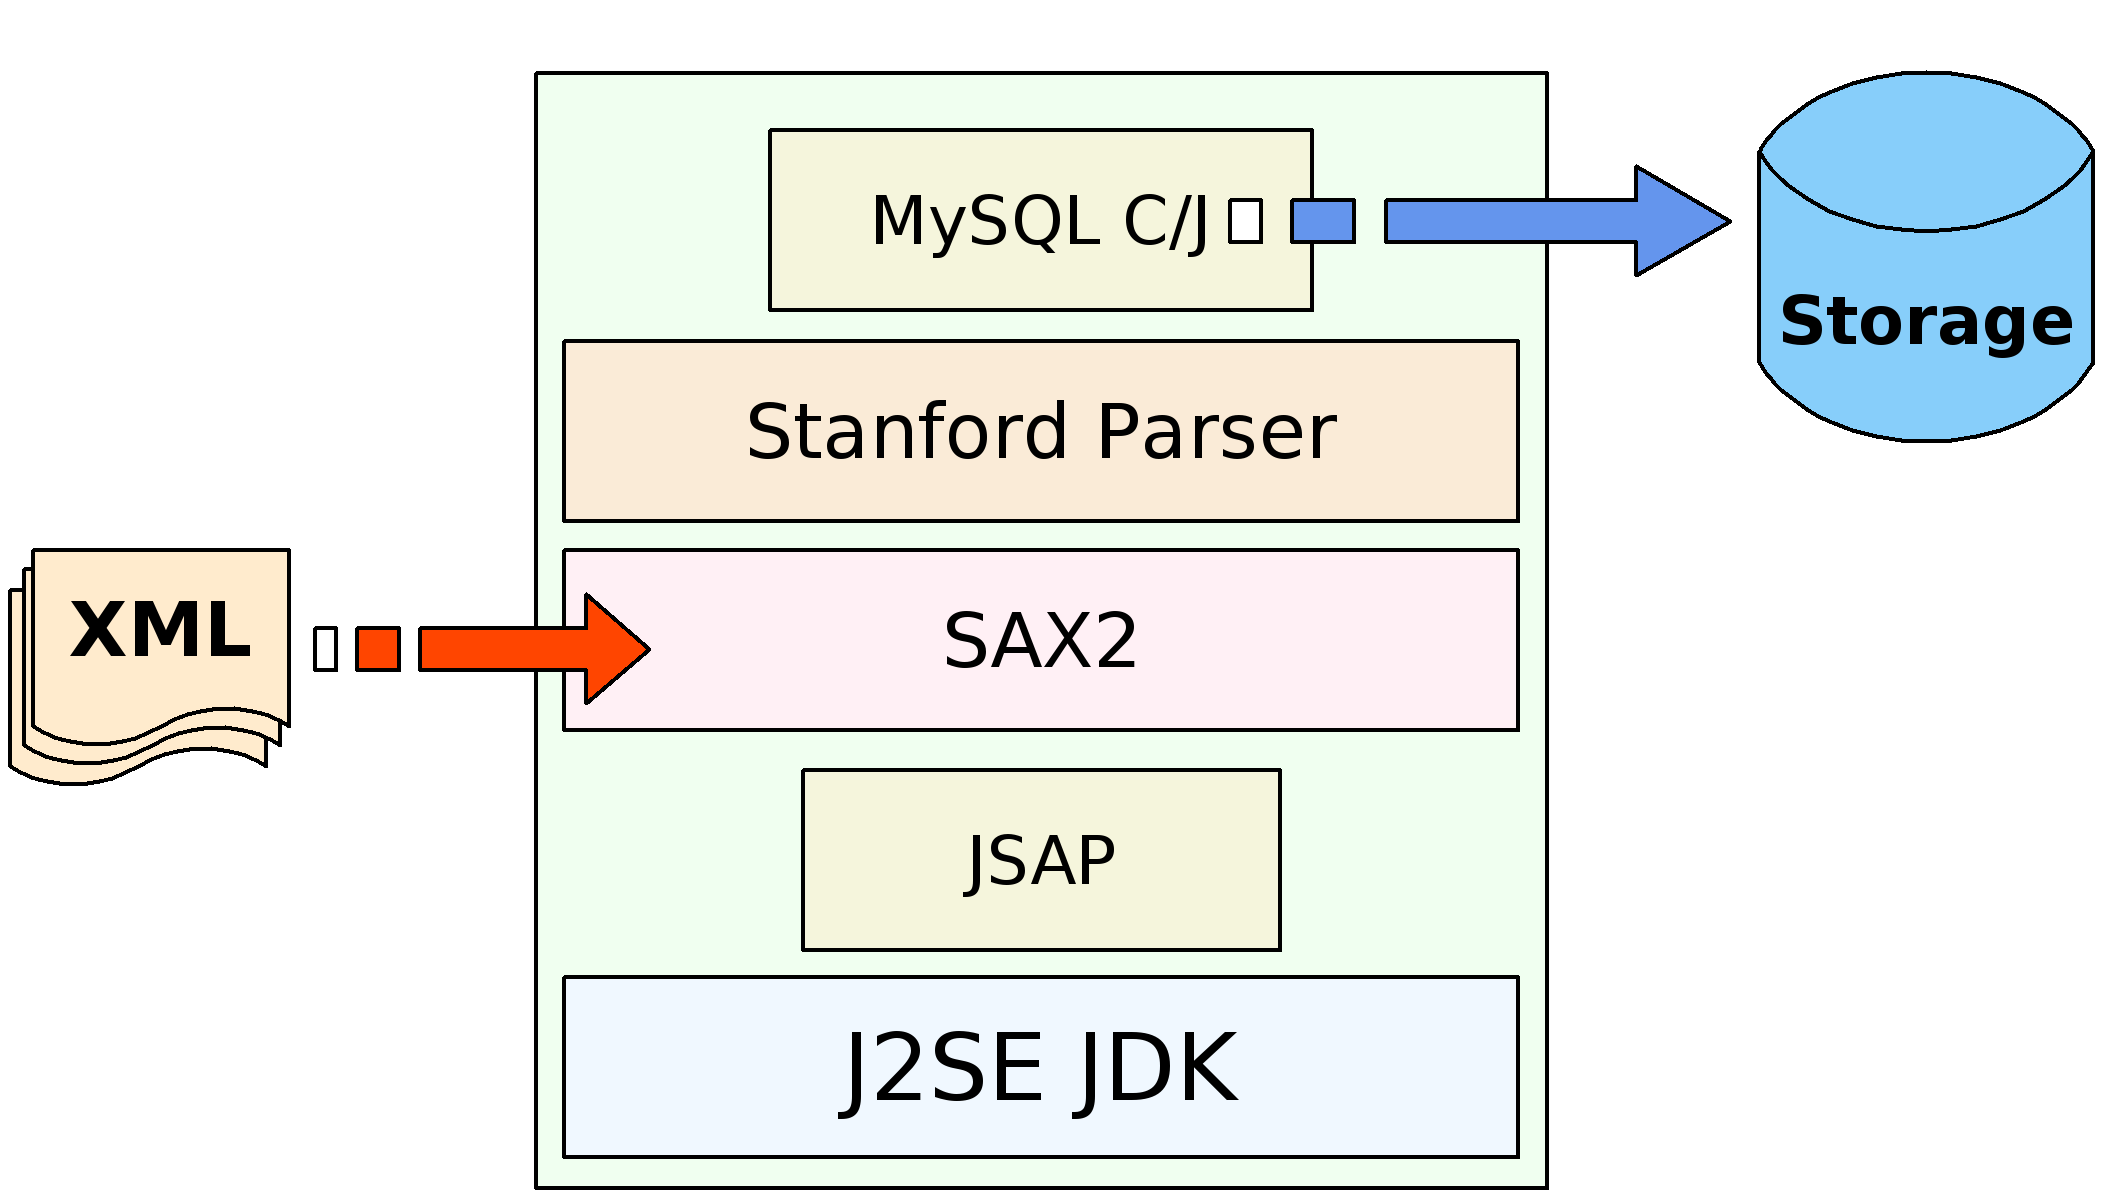
\includegraphics[scale=0.1425]{images/build/miex-libs.png}
    \end{center}
  \end{figure}
}

%-------------------------- SLIDE ---------------------------%

\frame
{
  \frametitle{Estructura de la BDD}

  \vspace{-0.4cm}

  \begin{figure}[h]
    \begin{center}
      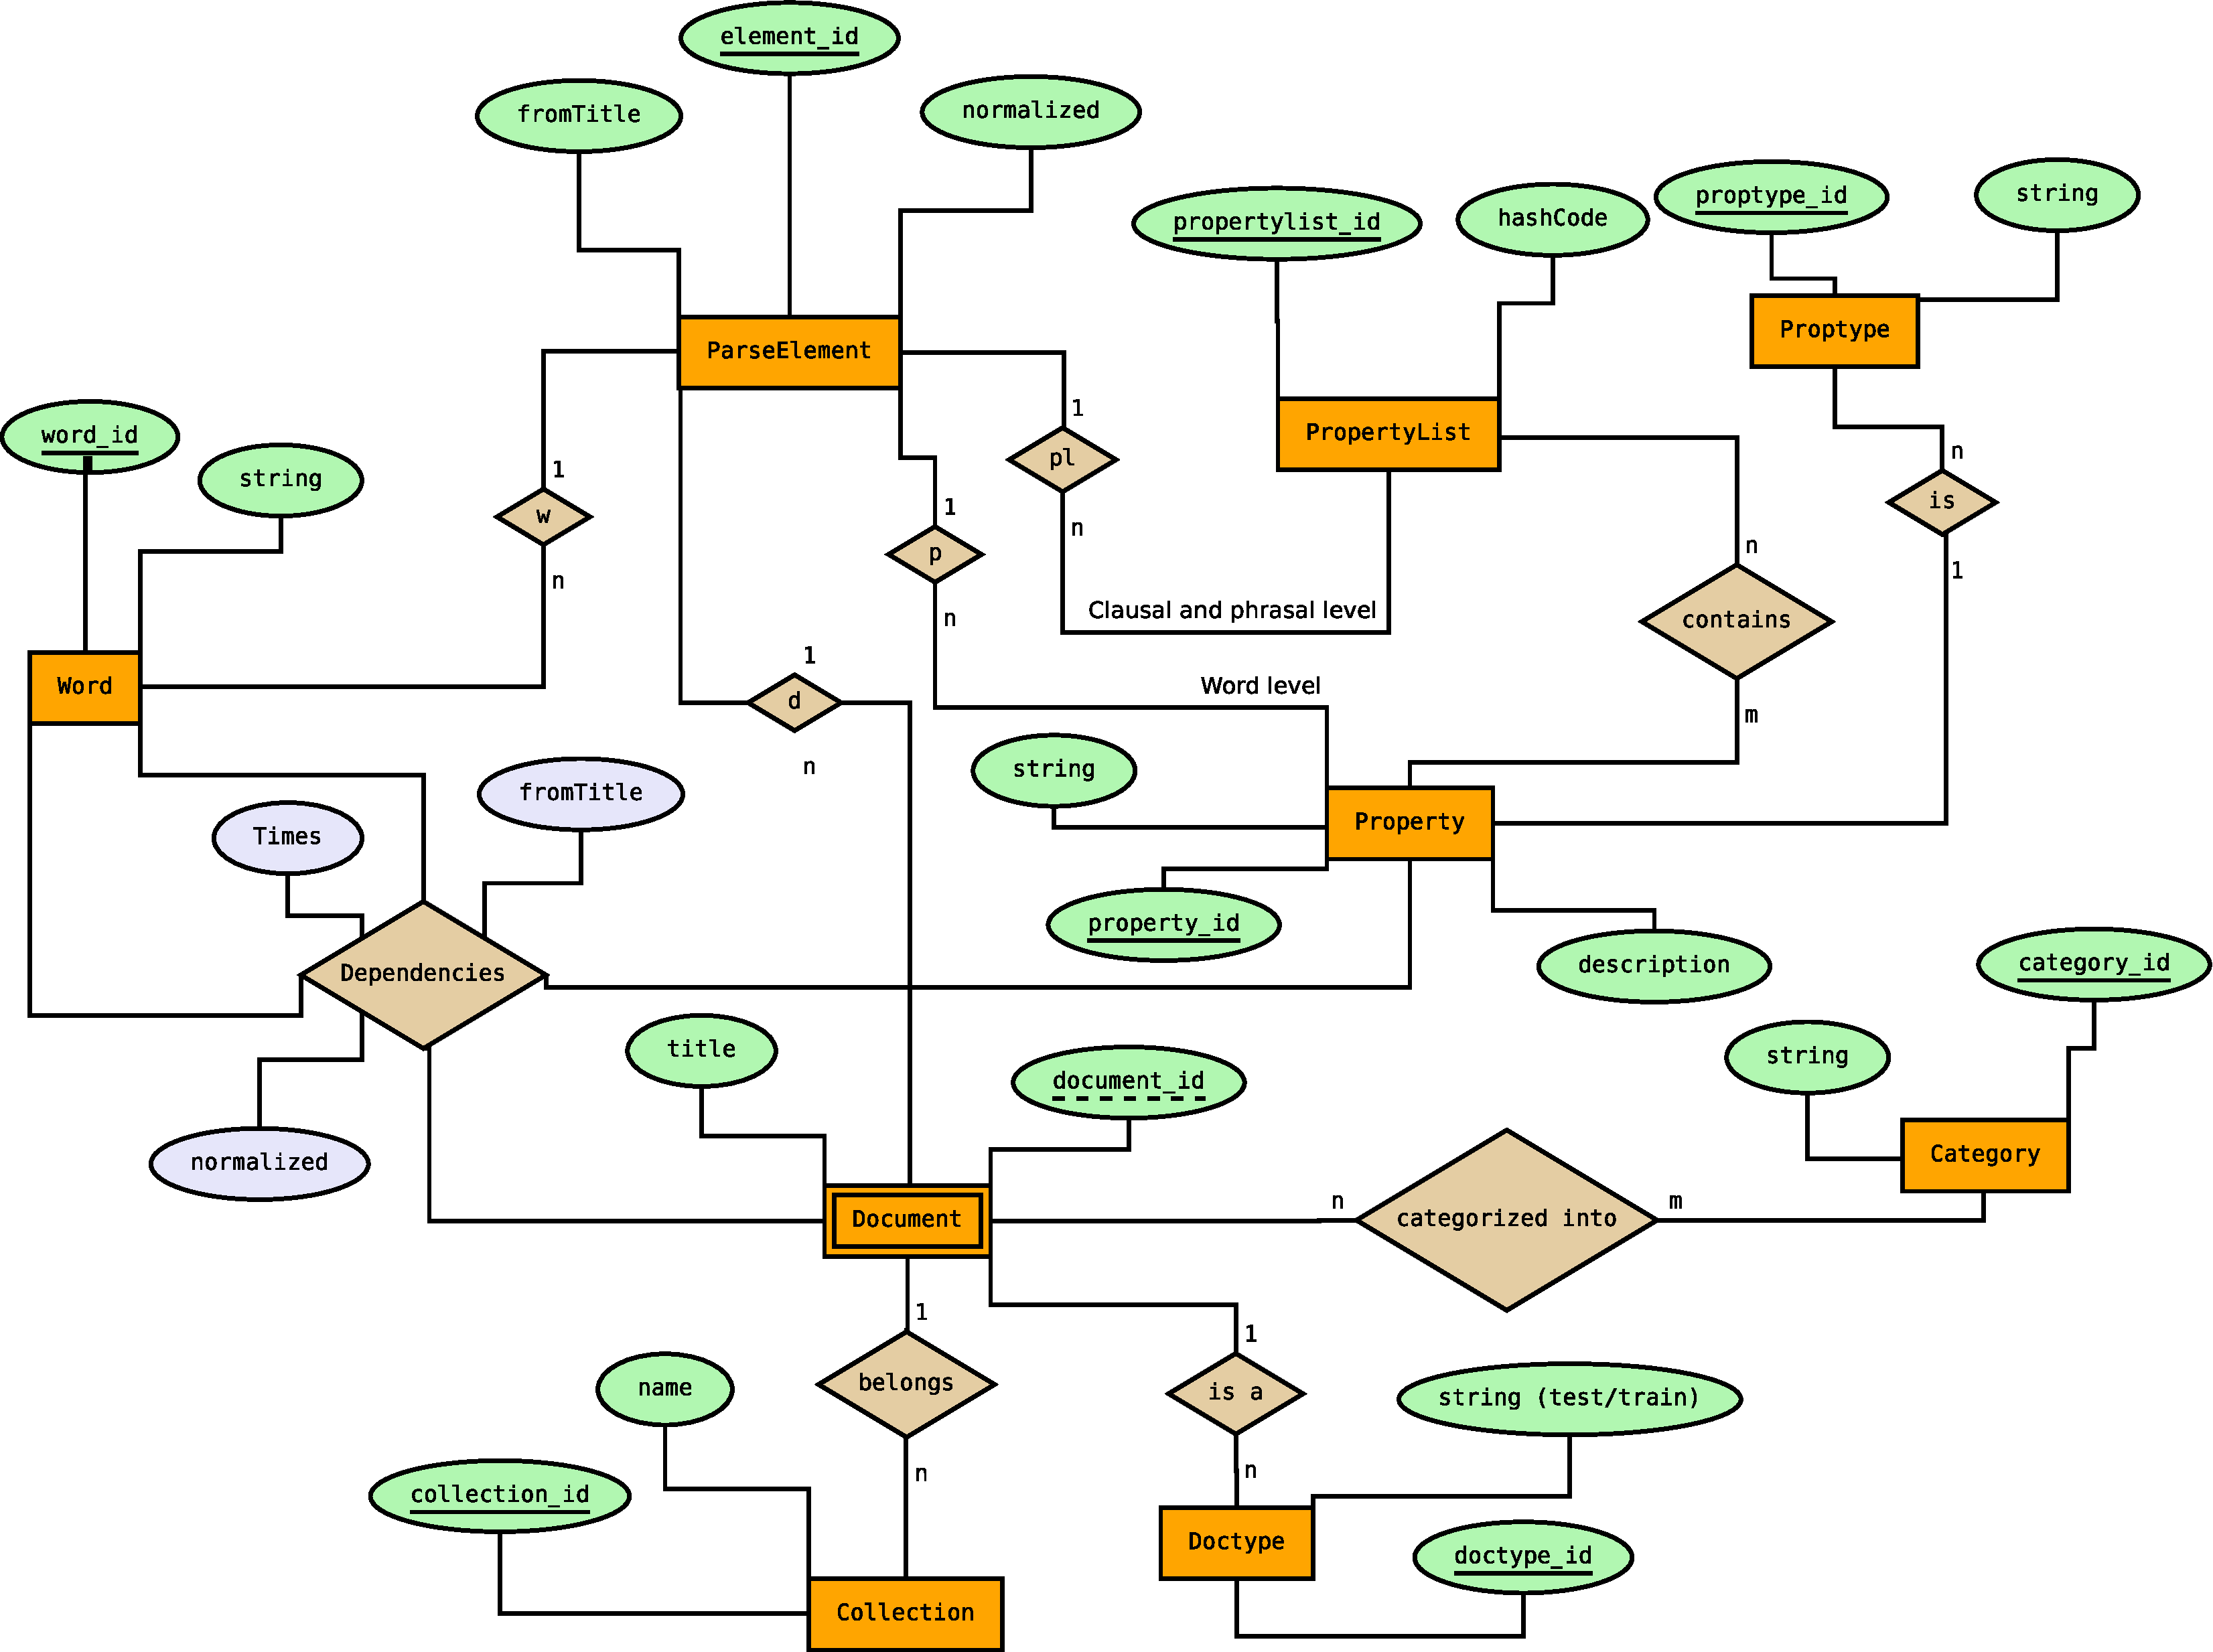
\includegraphics[scale=0.175]{images/bdd-e-r.pdf}
    \end{center}
  \end{figure}
}

%%%%%%%%%%%%%%%%%%%%%%%%%%%%%%%%%%%%%%%%%%%%%%%%%%%%%%%%%%%%%%%%%%%%%%%%%
% Recursos sobre el proyecto                                            %
%%%%%%%%%%%%%%%%%%%%%%%%%%%%%%%%%%%%%%%%%%%%%%%%%%%%%%%%%%%%%%%%%%%%%%%%%

\section{Recursos}

\frame
{
  \setcounter{tocdepth}{1}
  \tableofcontents[currentsection]
}


%%%%%%%%%%%%%%%%%%%%%%%%%%%%%%%%%%%%%%%%%%%%%%%%%%%%%%%%%%%%%%%%%%%%%%%%%
% Demo + Preguntas                                                      %
%%%%%%%%%%%%%%%%%%%%%%%%%%%%%%%%%%%%%%%%%%%%%%%%%%%%%%%%%%%%%%%%%%%%%%%%%

\section{Demo + Preguntas}

\frame
{
  \setcounter{tocdepth}{1}
  \tableofcontents[currentsection]
}

%-------------------------- SLIDE ---------------------------%

\frame
{

  \begin{center}

  {\fontfamily{augie}\fontsize{50}{52}\selectfont Demo}

  \end{center}

}

%-------------------------- SLIDE ---------------------------%

\frame
{
  \frametitle{Fin}

  \begin{beamerboxesrounded}[shadow=true]{}

  \begin{center}

  \Large{�Preguntas?}\\

  \end{center}

  \end{beamerboxesrounded}

  \vspace{1cm}

  %%%%

  \begin{beamerboxesrounded}[shadow=true]{Licencia}

  \begin{center}

  \small
  {
  GNU General Public License (versi�n 2)\\
  Fuentes en: http://miex.sf.net/
  }

  \end{center}

  \end{beamerboxesrounded}

  %%%%

  \begin{beamerboxesrounded}[shadow=true]{Tecnolog�a}

  \begin{center}

  \small
  {
  \LaTeX{} Beamer \scriptsize{http://latex-beamer.sf.net/}
  }

  \end{center}

  \end{beamerboxesrounded}

}

% That's all folks
\end{document}
